\subsection{System size dependence}
\label{sec:flow_sizedep}

\begin{figure}[!ht]
\begin{center}
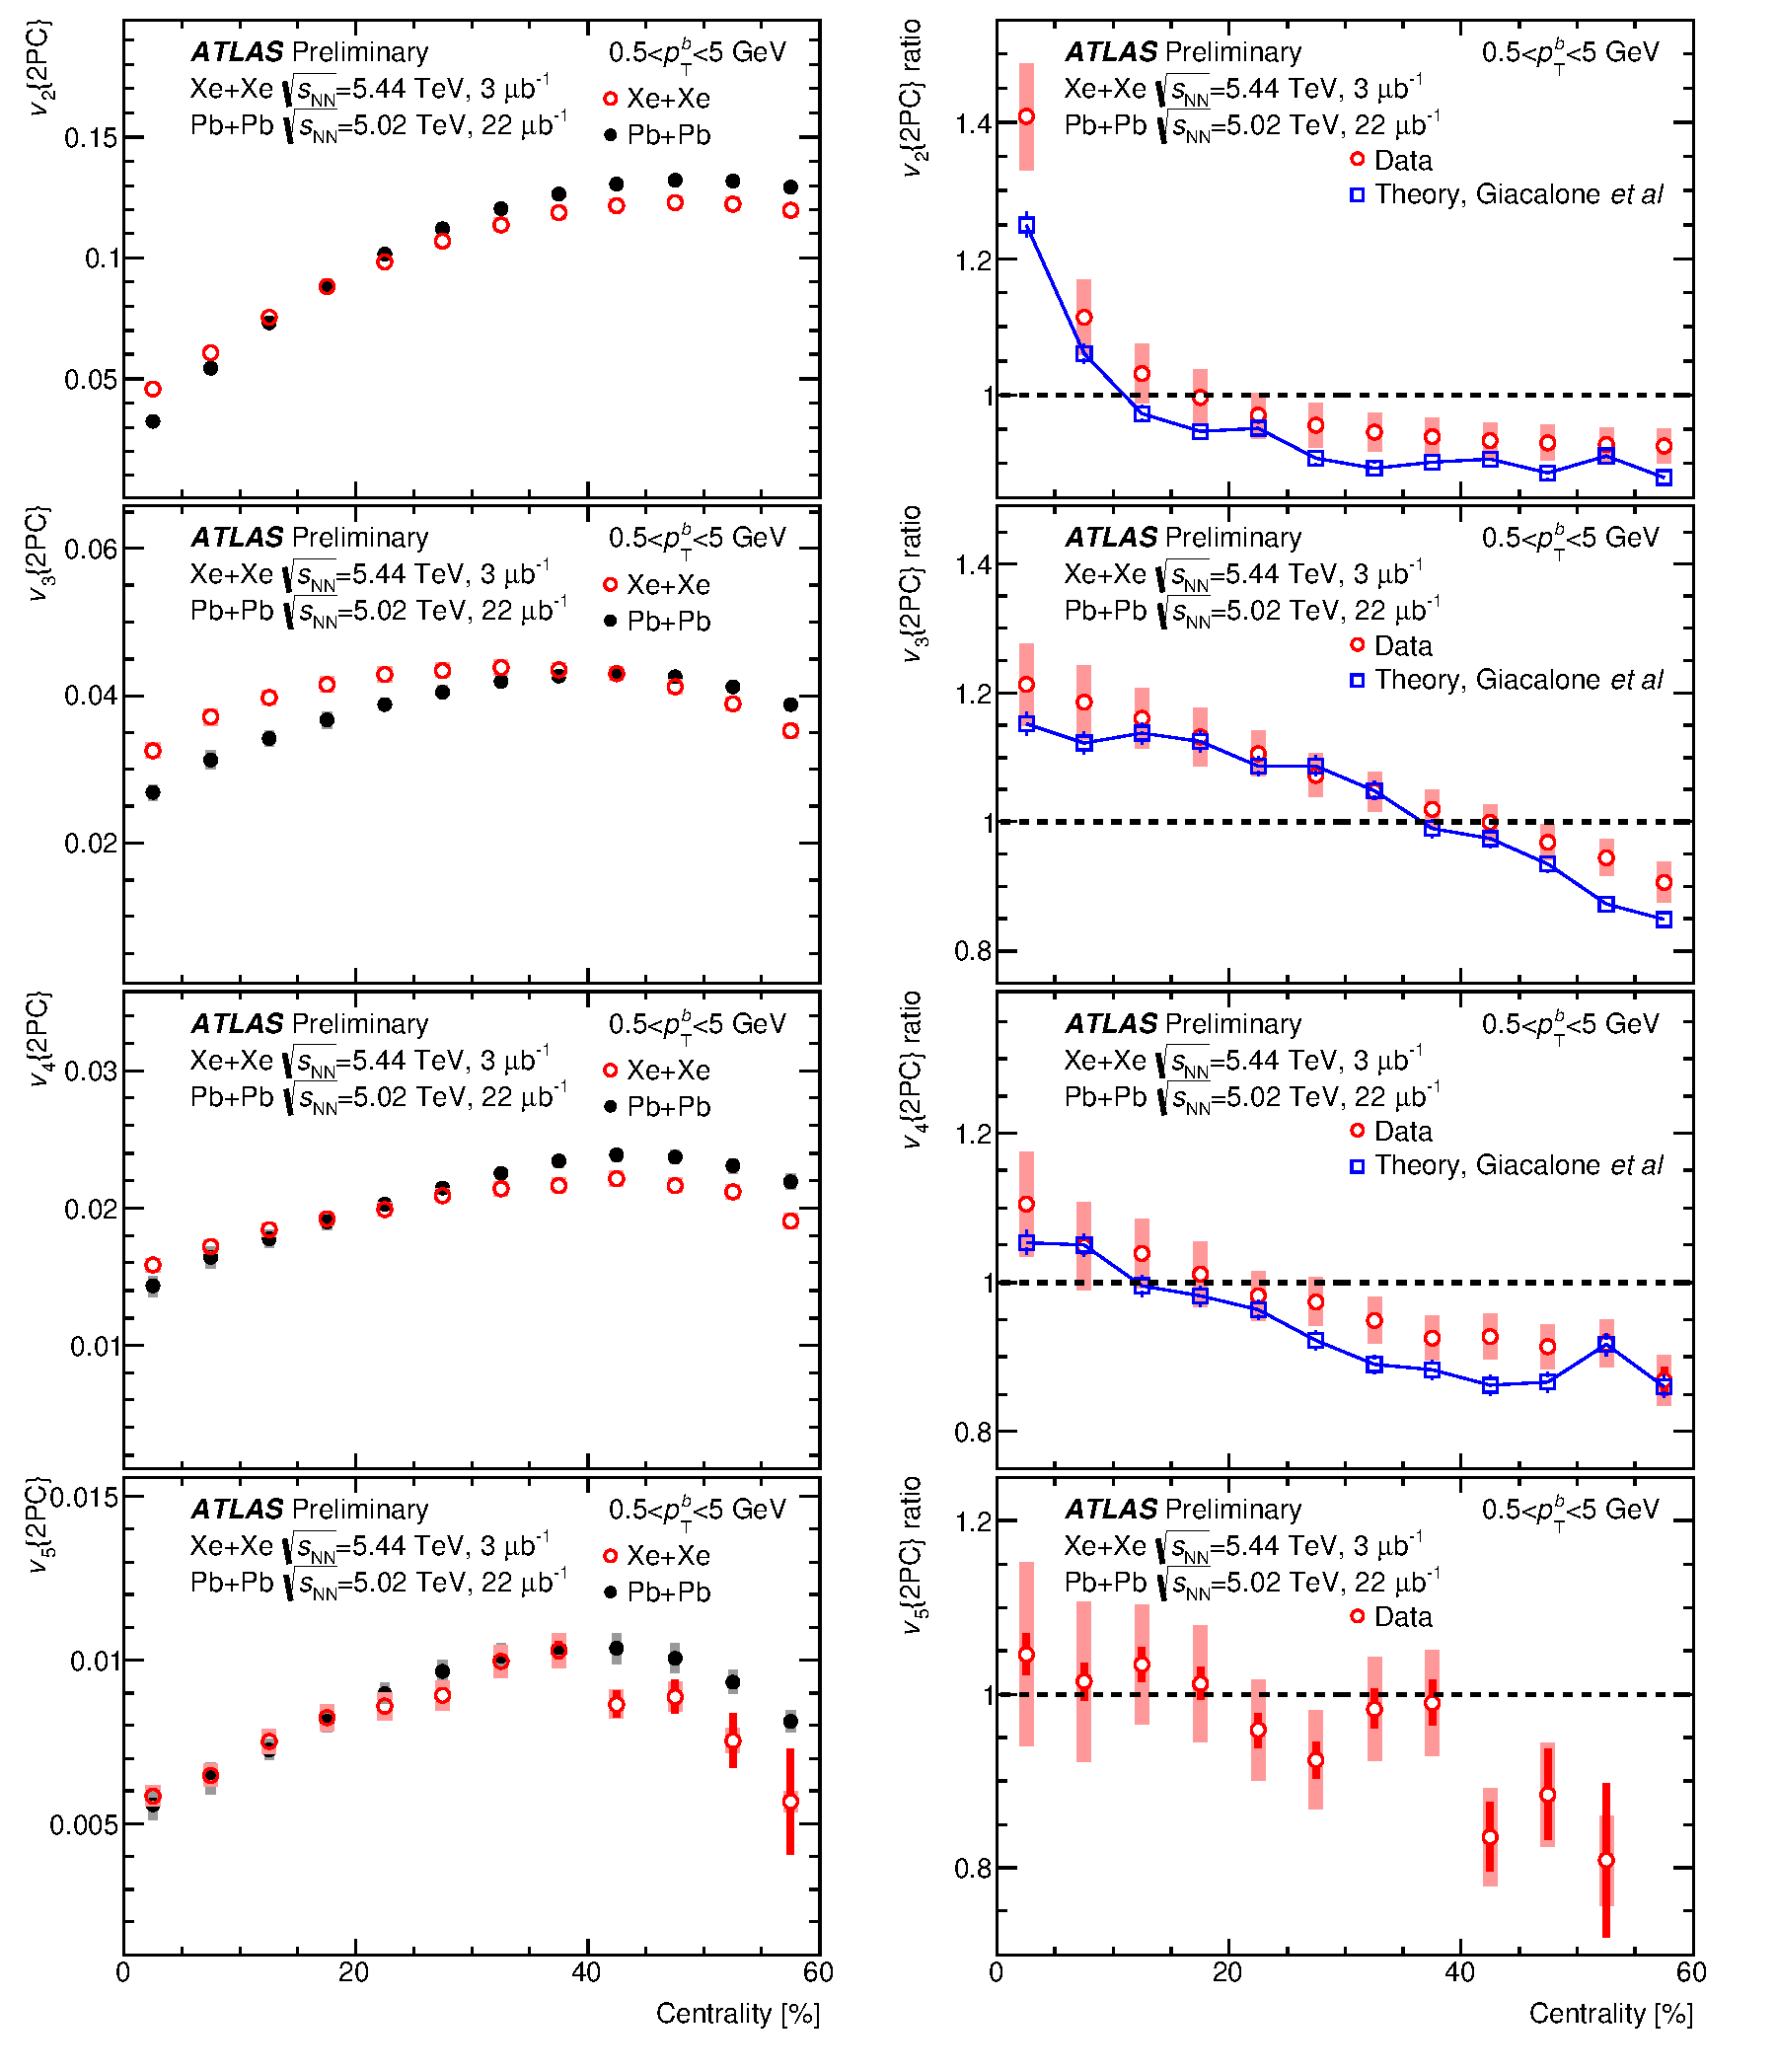
\includegraphics[width=0.8\textwidth]{\main/flow/figs/atlas_xexe_vn}
\caption{
Left panels: comparisons of the centrality dependence of the \vn\ measured 
  in \pbpb\ collisions at \snn=5.02~TeV to \xexe\ measurements. 
The plots are for the 0.5--5~GeV \pT\ interval. 
From top to bottom each row corresponds to a different harmonic order $n$.
The ratios are compared to theoretical predictions from Ref.~\cite{Giacalone:2017dud}.
ATLAS Data taken from Ref.~\cite{ATLAS-CONF-2018-011}.
}
\label{fig:atlas_xexe_vn}
\end{center}
\end{figure}

As pointed out previously, the \vn\ measurements are simultaneously
  sensitive to the initial collision geometry as well as to the 
  expansion dynamics of the QGP, which makes it difficult to 
  constrain either feature from the present \vn\ measurements.
Performing \vn\ measurements for several different colliding species
  at a comparable level of precision as the present LHC measurements,  
  could possibly constrain the prevailing combinations of initial-state 
  models and transport coefficients that reproduce the present \vn\ data 
  fairly well.
As a historical precedent at RHIC, the $v_2$ measurements in Cu+Cu 
  collisions lead to several interesting insights into heavy ion 
  collisions~\cite{RHIC_CU_CU}.
The Cu+Cu $v_2$ were found to be significantly larger that what was 
  expected a priori from the simplistic optical Glauber model~\cite{OPTICAL_GLAUBER}
  based calculations in use at the time.
This larger $v_2$ was realized to be the result of event-by-event fluctuations
  in the positions of the colliding nucleons, which leads to larger
  elliptic deformation in the initial geometry which in turn leads 
  to larger $v_2$.


Figure~\ref{fig:atlas_xexe_vn} shows ATLAS comparisons of the \vn\
  in \xexe\ and \pbpb\ collisions as a function of centrality (left panels)
  and their ratio (right panels).
Also shown for comparison in the right panels are theoretical predictions
  for the ratios from Ref.~\cite{Giacalone:2017dud}.
It is seen that for $v_2$ in central events, the \xexe\ values are
  considerably larger than the corresponding \pbpb\ values.
This is seen most clearly from the ratio plots.
With decreasing centrality the ratio for $v_2$ decreases faster and
  becomes smaller than one by the 10--15\% centrality interval.
For more peripheral events the ratio keeps decreasing but at a
  smaller rate and becomes roughly 0.9 by the 60--70\% centrality.
For $v_3$ the \xexe\ values are larger than the \pbpb\ values
  over the 0--30\% centrality interval,  become comparable over the
  30--40\% centrality interval and smaller for more peripheral events.
In this case the ratio in the 0--5\% most central events is smaller
  than for $v_2$, and decreases almost linearly over the 0--70\%
  centrality range.
For $v_4$ the \xexe\ values are only marginally larger in the top
  0--5\% central events.
The ratio for $v_4$ becomes comparable or less than one by the
  5--10\% centrality and continues to decrease for
  more peripheral events.
For $v_5$ the \xexe\ values are smaller throughout.
These trends can be explained as follows:
  \xexe\ being a smaller system than \pbpb, the effect of fluctuations
  is considerably more important.
The fluctuations increase the initial eccentricities of the collision
  geometry and this effect contributes to enhancing the \vn.
However, because \xexe\ is a smaller collision system the viscous
  effects (which suppress the \vn) are larger, and play a bigger role
  with decreasing centrality and increasing harmonic order.
In most central events, the effect of the increased fluctuations wins
  for $v_2$.
But with increasing harmonic order and/or decreasing centrality, 
  eventually the viscous effects reduce the \vn compared to \pbpb.
These observations indicate the ability of such cross-system 
  \vn\ measurements to be sensitive to initial conditions of 
  the heavy ion collision as well as the transport coefficients
  of the QGP. 
The measured ratios for the \vn(Xe--Xe)/\vn(\pbpb) are qualitatively reproduced 
  by the theory predictions from Ref.~\cite{Giacalone:2017dud},
	and are typically consistent with the measurements within 1--2$\sigma$
	uncertainties.
Therefore with the current set of measurements, this model cannot be validated
  or ruled out.
Figure~\ref{fig:atlas_xexe_vn} also shows predictions of the \vn\ ratios
  for Ar--Ar and O--O from the same theoretical model.
The predictions show considerably larger variation of the centrality dependence
  of the \vn\ going from \xexe$\rightarrow$Ar--Ar$\rightarrow$O--O, as compared to
	the variation going from \pbpb$\rightarrow$\xexe.
Given, such strong trends in the theory predictions, performing \vn\ measurements 
  in light ion species such as Ar--Ar and O--O in Run~3 can provide strong 
  constrains on the prevailing theoretical models.

Furthermore, there has been much work is studying long-range correlations
  observed in \pA~\cite{HION-2016-01,CMS:2012qk,Abelev:2012ola,HION-2012-13,HION-2013-04},
  d--A~\cite{Aidala:2017pup}, $^{3}\mathrm{He}$--A~\cite{Adare:2015ctn} 
  and more recently in \pp~\cite{HION-2015-09,HION-2016-01} collisions 
  (see Chapter~ref{chapter:smallsystems}).
Measuring flow in medium and light ions would allow for a continuous study 
  of how collective phenomena vary going from large (\pbpb) to small 
  (\pA\ and \pp) systems and lead to a better understanding of collectivity
  in small systems.


